%% BioMed_Central_Tex_Template_v1.06
%%                                      %
%  bmc_article.tex            ver: 1.06 %
%                                       %

%%IMPORTANT: do not delete the first line of this template
%%It must be present to enable the BMC Submission system to
%%recognise this template!!

%%%%%%%%%%%%%%%%%%%%%%%%%%%%%%%%%%%%%%%%%
%%                                     %%
%%  LaTeX template for BioMed Central  %%
%%     journal article submissions     %%
%%                                     %%
%%          <8 June 2012>              %%
%%                                     %%
%%                                     %%
%%%%%%%%%%%%%%%%%%%%%%%%%%%%%%%%%%%%%%%%%


%%%%%%%%%%%%%%%%%%%%%%%%%%%%%%%%%%%%%%%%%%%%%%%%%%%%%%%%%%%%%%%%%%%%%
%%                                                                 %%
%% For instructions on how to fill out this Tex template           %%
%% document please refer to Readme.html and the instructions for   %%
%% authors page on the biomed central website                      %%
%% http://www.biomedcentral.com/info/authors/                      %%
%%                                                                 %%
%% Please do not use \input{...} to include other tex files.       %%
%% Submit your LaTeX manuscript as one .tex document.              %%
%%                                                                 %%
%% All additional figures and files should be attached             %%
%% separately and not embedded in the \TeX\ document itself.       %%
%%                                                                 %%
%% BioMed Central currently use the MikTex distribution of         %%
%% TeX for Windows) of TeX and LaTeX.  This is available from      %%
%% http://www.miktex.org                                           %%
%%                                                                 %%
%%%%%%%%%%%%%%%%%%%%%%%%%%%%%%%%%%%%%%%%%%%%%%%%%%%%%%%%%%%%%%%%%%%%%

%%% additional documentclass options:
%  [doublespacing]
%  [linenumbers]   - put the line numbers on margins

%%% loading packages, author definitions

%\documentclass[twocolumn]{bmcart}% uncomment this for twocolumn layout and comment line below
\documentclass{bmcart}

%%% Load packages
\usepackage{amsthm,amsmath,amssymb,amsfonts}
\usepackage{algorithm,algorithmic}
%\RequirePackage{natbib}
%\RequirePackage[authoryear]{natbib}% uncomment this for author-year bibliography
\usepackage{graphicx}
\usepackage{tabularx}
\usepackage{multirow}
\usepackage{paralist}
\usepackage{gensymb}
\RequirePackage{hyperref}
\usepackage[utf8]{inputenc} %unicode support
%\usepackage[applemac]{inputenc} %applemac support if unicode package fails
%\usepackage[latin1]{inputenc} %UNIX support if unicode package fails

%%%%%%%%%%%%%%%%%%%%%%%%%%%%%%%%%%%%%%%%%%%%%%%%%
%%                                             %%
%%  If you wish to display your graphics for   %%
%%  your own use using includegraphic or       %%
%%  includegraphics, then comment out the      %%
%%  following two lines of code.               %%
%%  NB: These line *must* be included when     %%
%%  submitting to BMC.                         %%
%%  All figure files must be submitted as      %%
%%  separate graphics through the BMC          %%
%%  submission process, not included in the    %%
%%  submitted article.                         %%
%%                                             %%
%%%%%%%%%%%%%%%%%%%%%%%%%%%%%%%%%%%%%%%%%%%%%%%%%

%\def\includegraphic{}
%\def\includegraphics{}


%%% Put your definitions there:
\startlocaldefs

\newenvironment{Algorithm}[1]{\begin{minipage}{0.45\textwidth}\centering\begin{minipage}{#1}\begin{algorithm}[H]}{\end{algorithm}\end{minipage}\end{minipage}}

\newcommand{\tickYes}{\checkmark}

\newcommand{\INDSTATE}[1][1]{\STATE\hspace{#1\algorithmicindent}}

\endlocaldefs


%%% Begin ...
\begin{document}

%%% Start of article front matter
\begin{frontmatter}

\begin{fmbox}
\dochead{Research}

%%%%%%%%%%%%%%%%%%%%%%%%%%%%%%%%%%%%%%%%%%%%%%
%%                                          %%
%% Enter the title of your article here     %%
%%                                          %%
%%%%%%%%%%%%%%%%%%%%%%%%%%%%%%%%%%%%%%%%%%%%%%

\title{Utilising User Judgement of Direction for Locating Interface Positions}

%%%%%%%%%%%%%%%%%%%%%%%%%%%%%%%%%%%%%%%%%%%%%%
%%                                          %%
%% Enter the authors here                   %%
%%                                          %%
%% Specify information, if available,       %%
%% in the form:                             %%
%%   <key>={<id1>,<id2>}                    %%
%%   <key>=                                 %%
%% Comment or delete the keys which are     %%
%% not used. Repeat \author command as much %%
%% as required.                             %%
%%                                          %%
%%%%%%%%%%%%%%%%%%%%%%%%%%%%%%%%%%%%%%%%%%%%%%

\author[
   addressref={aff1},                   % id's of addresses, e.g. {aff1,aff2}
   corref={aff1},                       % id of corresponding address, if any
%   noteref={n1},                        % id's of article notes, if any
   email={j.a.mcnaughton@durham.ac.uk}   % email address
]{\inits{JM}\fnm{James} \snm{McNaughton}}
\author[
   addressref={aff2},
   email={tcrick@cardiffmet.ac.uk}
]{\inits{TC}\fnm{Tom} \snm{Crick}}

%%%%%%%%%%%%%%%%%%%%%%%%%%%%%%%%%%%%%%%%%%%%%%
%%                                          %%
%% Enter the authors' addresses here        %%
%%                                          %%
%% Repeat \address commands as much as      %%
%% required.                                %%
%%                                          %%
%%%%%%%%%%%%%%%%%%%%%%%%%%%%%%%%%%%%%%%%%%%%%%


\address[id=aff1]{%                           % unique id
  \orgname{School of Education, Durham University}, % university, etc
  \street{South Road},                     %
  \postcode{DH1 3LE}                                % post or zip code
  \city{Durham},                              % city
  \cny{UK}                                    % country
}
\address[id=aff2]{%
  \orgname{Department of Computing \& Information Systems, Cardiff Metropolitan University},
  \street{Western Avenue},
  \postcode{CF5 2YB}
  \city{Cardiff},
  \cny{UK}
}

%%%%%%%%%%%%%%%%%%%%%%%%%%%%%%%%%%%%%%%%%%%%%%
%%                                          %%
%% Enter short notes here                   %%
%%                                          %%
%% Short notes will be after addresses      %%
%% on first page.                           %%
%%                                          %%
%%%%%%%%%%%%%%%%%%%%%%%%%%%%%%%%%%%%%%%%%%%%%%

\begin{artnotes}
%\note{Sample of title note}     % note to the article
%\note[id=n1]{Equal contributor} % note, connected to author
\end{artnotes}

\end{fmbox}% comment this for two column layout

%%%%%%%%%%%%%%%%%%%%%%%%%%%%%%%%%%%%%%%%%%%%%%
%%                                          %%
%% The Abstract begins here                 %%
%%                                          %%
%% Please refer to the Instructions for     %%
%% authors on http://www.biomedcentral.com  %%
%% and include the section headings         %%
%% accordingly for your article type.       %%
%%                                          %%
%%%%%%%%%%%%%%%%%%%%%%%%%%%%%%%%%%%%%%%%%%%%%%

\begin{abstractbox}

\begin{abstract} % abstract
% \parttitle{First part title} %if any
% Text for this section.
% \parttitle{Second part title} %if any
% Text for this section.

In many co-located, collaborative systems there is a need for the devices used to be informed of the positions of their linked devices in a physical environment.
This paper presents a novel method of utilising users' judgement of direction to attain the location and orientation of a direct touch interface.
The technique requires a user to create several arrows on an interface which point towards physical landmarks in an environment.
This allows for the setup of interface locations which is: \begin{inparaenum}[(i)] \item quick, \item inexpensive, \item not encumbering and \item capable of being performed despite obstructions in the environment\end{inparaenum}.
A user study is presented which investigates what influence a user's accuracy has on the resulting calculated location of an interface.
The study reveals that the magnitude of a user's inaccuracies is proportional to the size of the error in the technique's result.
\end{abstract}

%%%%%%%%%%%%%%%%%%%%%%%%%%%%%%%%%%%%%%%%%%%%%%
%%                                          %%
%% The keywords begin here                  %%
%%                                          %%
%% Put each keyword in separate \kwd{}.     %%
%%                                          %%
%%%%%%%%%%%%%%%%%%%%%%%%%%%%%%%%%%%%%%%%%%%%%%

\begin{keyword}
\kwd{TBC}
\end{keyword}

% MSC classifications codes, if any
%\begin{keyword}[class=AMS]
%\kwd[Primary ]{}
%\kwd{}
%\kwd[; secondary ]{}
%\end{keyword}

\end{abstractbox}
%
%\end{fmbox}% uncomment this for twcolumn layout

\end{frontmatter}

%%%%%%%%%%%%%%%%%%%%%%%%%%%%%%%%%%%%%%%%%%%%%%
%%                                          %%
%% The Main Body begins here                %%
%%                                          %%
%% Please refer to the instructions for     %%
%% authors on:                              %%
%% http://www.biomedcentral.com/info/authors%%
%% and include the section headings         %%
%% accordingly for your article type.       %%
%%                                          %%
%% See the Results and Discussion section   %%
%% for details on how to create sub-sections%%
%%                                          %%
%% use \cite{...} to cite references        %%
%%  \cite{koon} and                         %%
%%  \cite{oreg,khar,zvai,xjon,schn,pond}    %%
%%  \nocite{smith,marg,hunn,advi,koha,mouse}%%
%%                                          %%
%%%%%%%%%%%%%%%%%%%%%%%%%%%%%%%%%%%%%%%%%%%%%%

%%%%%%%%%%%%%%%%%%%%%%%%% start of article main body
% <put your article body there>

%%%%%%%%%%%%%%%%
%% Background %%
%%

\section*{Introduction}\label{sec:intro}

Direct-touch interfaces provide an effective digital medium in which people can collaborate on various tasks, including learning~\cite{Marshall2007a,Marshall2008}. 
Research regarding collaboration on direct-touch interfaces is generally focused on collaboration between multiple participants across a single interface~\cite{Piper2009,Rick2009,Ryall2006a}. 
However, when multiple interfaces capable of interacting with each other are used, an opportunity arises for collaboration between participants at different interfaces.
This use of multiple interfaces in a shared environment can be beneficial for collaboration~\cite{Wallace2008a,Wallace2009}.

The physical locations of interfaces can be used to aid tasks involving interaction between linked devices.
For example, the Interactive Workspaces project~\cite{Johanson2002} generates a map of interface locations.
This map is used to facilitate collaboration between the multiple interfaces.
Users can pass materials between the interfaces using their knowledge of their physical positions.
When a material transfer is initiated the system can use the direction defined by the user and the generated map to find the interface the materials should be sent to.

\begin{figure}[h!]
   \centering
   \caption{An example of how content items can be transferred between linked interfaces using flicking.}
   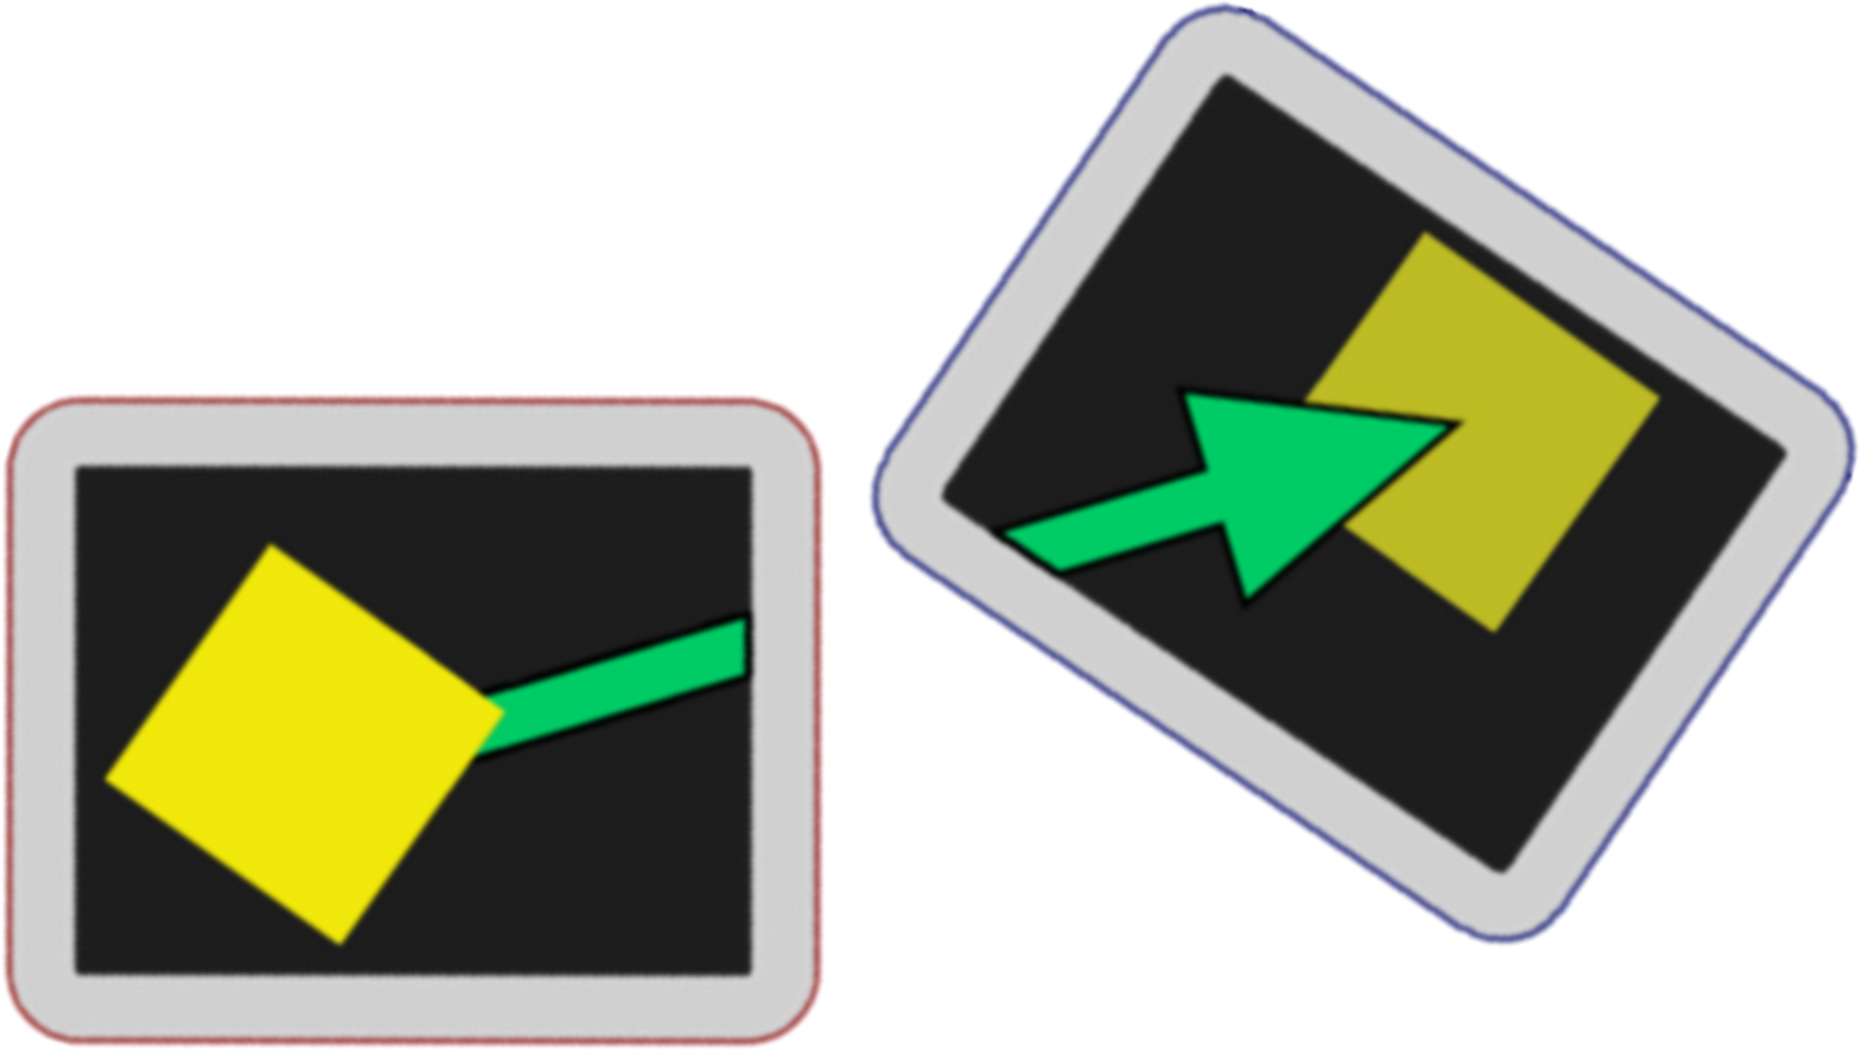
\includegraphics[width=0.4\textwidth]{figures/flicking.png}
   \label{fig:flick}
\end{figure}

Activities of content sharing in multi-interface environments are becoming more common~\cite{Nacenta2009}.
Another example of where the knowledge of interface locations facilitates the passing of materials between separate devices originates from the SynergySpace project~\cite{Burd2009}.
The software framework built for SynergySpace is intended for use on direct-touch interfaces, specifically multi-touch tabletops.
This allows the system to allow users to perform a flicking~\cite{Reetz2006} motion to transfer content.
Users flick a content item in the direction of the interface they wish to send content to.
The item travels off the side of the initial interface and appears on the target interface as shown in Figure \ref{fig:flick}.
When the item arrives on the target interface, the framework can use its knowledge of the interface locations to ensure the item travels into view from the direction of the source interface.
This is intended to aid users in identifying where newly arrived content items were sent from.

Both the Interactive Workspaces~\cite{Johanson2002} and SynergySpace~\cite{Burd2009} projects indicate that the ability for an interface to have knowledge of its location relative to linked interfaces surrounding it can be beneficial.
Another example of the benefits of an interface knowing its location originates from a system which uses multiple projectors where projected outputs overlap.
The outputs are seamlessly stitched together by the system to give the appearance of a single projection.
In order for this to be achieved the system must have information regarding the relative positions of each projected output.
The stitching of multiple projector outputs to create large public displays is becoming much more frequent~\cite{Jones2011}.
Each system which utilises the stitching of visual outputs needs a method of attaining their locations.

With systems requiring knowledge of the locations of their interfaces, a method of obtaining this positional information is needed.
It is possible to measure the location and orientation of an interface using physical tools like rulers and protractors. 
Because of the time consuming nature of this manual measurement strategy it is best suited for an environment in which the interfaces remain in a fixed position for long periods of time.

However, there are scenarios in which the interfaces may be moved on a regular basis.
For example, the SynergySpace project~\cite{Burd2009} is intended for classroom environments.
These classroom environments are physical spaces in which furniture is frequently moved or rearranged to accommodate different learning activities during the course of a day~\cite{Tiburcio2005}.
Therefore, it is likely that any interfaces in the environment used by the system will not remain in fixed positions.
Measuring the locations and angles of each interface in the environment directly, then inputting this information into the system will take time on every reconfiguration of the environment.
In this time the system will not function as intended because the system's knowledge concerning the positions of interfaces will be incorrect.

Incorrect knowledge of interface positions is problematic for systems which use the information to stitch multiple visual outputs~\cite{Dietz2004,Jones2011}.
The image displayed by a repositioned interface would no longer align with the output from other linked interfaces and therefore would not be appropriately stitched.

Therefore, a method of obtaining the position of an interface quickly, without the need for time consuming measurements, is required.


\section*{Background}\label{sec:related}

Obtaining the position of an interface can be achieved through technological means.
The use of RFID chips~\cite{Ni2004} is one such technological approach.
These devices are inexpensive and can be used to get the positional information of the object they are attached to.
However, the accuracy of locations given by RFID chips is dependent on the number of sensors in an environment.
Despite the relatively low cost of the chips, the large number of sensors needed for accurate readings can be expensive.
Also, the addition of more sensors requires the system to spend more time compiling the locational information for each RFID chip detected~\cite{Ni2004}.
The same trade-off between expense and accuracy is also present for similar technologies using electro-magnetic waves, such as Wi-Fi~\cite{Cheng2005}.

Infra-red sensors can be used to attain the locations of interfaces~\cite{Kortuem2005}.
By detecting the relative location and strength of known infra-red light sources, a device with infra-red sensors can determine its position.
However, the technology is very sensitive and small changes in the light level can result in the calculated location varying from the sensors' actual locations to a large extent~\cite{Kortuem2005}.
This technology can also be affected by obstruction.
An object blocking an infra-red sensor's view of one or more infra-red light sources can result in the system obtaining incorrect positional information.
Therefore, for this technology to be used in a system, the environment must be clear of obstruction and have a consistent light level.
These two restraints make this technology suitable for only a small number of scenarios.

Visible light can be used for detecting the location of an interface~\cite{Lee2004}.
Using light sensing technology, an interface can detect its location by using patterns projected from a light source.
However, like infra-red sensors~\cite{Kortuem2005}, these visible light sensors require a clear line of sight to the light source.
If obstructed, a sensor's reading would result in the incorrect calculation of its location.

Visual markers called fiducials~\cite{Bose1990}, which are often used in augmented reality systems, could also be used for obtaining the position of an interface.
A camera is used to identify and locate the markers which each carry a unique pattern that the system can identify.
Several markers positioned on or around an interface could be located by a fiducial recognition system.
However, this technology requires a clear line of sight between the camera and the fiducials.
Like other location sensing technologies~\cite{Lee2004,Kortuem2005,Ni2004}, obstructions around the interface can cause inaccurate results.

When attempting to attain the location of an interface, an alternative to the use of sensing technologies is to utilise a technique driven by user input.
An example of this alternative method is where users measure the locations of the interface directly and input the information into the system through text entry. 
User inputs do have the disadvantage of relying on the accuracy of the users whereas sensing technologies can be relied on to be precise to a certain extent.
The accuracy of users can be influenced by a range of factors which would not affect the accuracy of sensing technologies, such as the magnitude of the distances being measured~\cite{Al-Imam2006}.
An inaccurate user-generated measurement, input as part of a location determining technique, would result in the calculated position of the interface being incorrect.
Therefore, it is important to take into consideration the accuracy of users when utilising techniques which rely on their inputs.

Observations on each technique discussed in this section show that each has strengths and weaknesses.
For example, a number of technology-based location sensing techniques discussed~\cite{Bose1990,Lee2004,Kortuem2005,Ni2004} will produce inaccurate locational information if obstruction of their sensing components occurs.
This is undesirable in any scenarios where obstruction may frequently occur.
For example, environments in which many users may be present around the interfaces would be unsuitable for these technologies.
A user may stand between the sensors and emitters used by the technologies to derive positional information.
This highlights how the weaknesses of a technique may make it use undesirable for some scenarios.

The technologies discussed in this section ~\cite{Bose1990,Lee2004,Kortuem2005,Ni2004} could also be considered unsuitable for systems in which the interface has no physical presence, such as those which use a projected output~\cite{Dietz2004,Jones2011}.
The projected output of a system has no physical presence other than the surface it is projected onto.
Several of the location sensing technologies discussed require an emitter or sensing device to be connected to the object being located ~\cite{Lee2004,Kortuem2005,Ni2004}.
However, this is not feasible for systems where the interface is projected.
The sensing device could be attached to the surface onto which the output is projected, but the repositioning of the output would require the sensing device to be repositioned separately which can be time consuming.
A camera could be used to attain the locations of the projected interfaces as discussed by Dietz et al.~\cite{Dietz2004}.
The projected output could also create virtual fiducial ~\cite{Bose1990} representations which can be located by a camera.
However, for both of these solutions, obstruction of the camera would result in inaccurate positional information being created.
Again, this highlights how the strengths and weaknesses of a position obtaining technique determine its suitability to a specific scenario.
Therefore it is important to compare the attributes of each technique when considering their use in a specific scenario.


% \section*{Tables}
% \begin{table}[h!]
% \caption{Sample table title. This is where the description of the table should go.}
%       \begin{tabular}{cccc}
%         \hline
%            & B1  &B2   & B3\\ \hline
%         A1 & 0.1 & 0.2 & 0.3\\
%         A2 & ... & ..  & .\\
%         A3 & ..  & .   & .\\ \hline
%       \end{tabular}
% \end{table}

\begin{table}[ht]
\centering
\caption{Comparison between the attributes of several position obtaining techniques.}
\begin{tabular}
{!{\vrule width 1.5pt}c|r!{\vrule width 1.5pt}c|c|c|c|c!{\vrule width 1.5pt}}
\noalign{\hrule height 1.5pt}
\multicolumn{2}{!{\vrule width 1.5pt}c!{\vrule width 1.5pt}}{ }
								&Obstruction 		&\multirow{2}{*}{Quick} 	&\multirow{2}{*}{Accurate} 	&\multirow{2}{*}{Inexpensive}		&Not				\\
\multicolumn{2}{!{\vrule width 1.5pt}c!{\vrule width 1.5pt}}{ }
								&Tolerant 			&		 				&							&								&Encumbering		\\
\noalign{\hrule height 1.5pt}
\multirow{4}{*}{\textbf{Technology}}
&RFID~\cite{Ni2004}				&\tickYes			&\tickYes				&\hspace{1.75cm}			&\hspace{1.75cm}				&\hspace{1.75cm}	\\
\cline{2-7}
&Infra-red~\cite{Kortuem2005}		&\hspace{1.75cm} 	&\tickYes				&\tickYes 					&								&					\\
\cline{2-7}
&Visible light~\cite{Lee2004}		&		 			&\tickYes				&\tickYes 					&								&\tickYes			\\
\cline{2-7}
&Fiducials~\cite{Bose1990}		&		 			&\tickYes				&\tickYes 					&								&\tickYes			\\
\cline{1-7}
\textbf{User Input}	
&Direct Measurement				&\tickYes			&\hspace{1.8cm}			&\tickYes					&\tickYes 						&\tickYes			\\
\noalign{\hrule height 1.5pt}
\end{tabular}
\label{table:techniquesComparison}
\end{table}

Table \ref{table:techniquesComparison} compares the attributes of the position obtaining techniques discussed in this section.
Each attribute listed in the comparison is derived from observations relating to the strengths and weaknesses of the techniques;

\begin{itemize}
  \item If a technique is able to give reliable results despite obstructions surrounding an interface it is deemed \textit{Obstruction Tolerant}.
  \item If the time taken to perform a technique is less than the time taken to measure the locations directly by hand it is deemed \textit{Quick}.
  \item If a technique produces usable positional information it is deemed \textit{Accurate}.
  \item If a technique does not require additional hardware to be purchased it is deemed \textit{Inexpensive}.
  \item If a technique does not require an additional physical device to be attached to the interface it is deemed to be \textit{Not Encumbering}.
\end{itemize}

For each technology discussed in this section a tick is given under each heading it conforms to.
In addition to the technologies discussed in this section, the user input based technique of directly measuring the location of the interfaces is also included.

Table \ref{table:techniquesComparison} shows that none of the position obtaining techniques discussed are without a weakness.
The majority of the technology based techniques have issues regarding obstruction which makes them unsuitable for use in the classroom scenario, discussed in Section \ref{sec:intro}.
This is due to the potential obscuring of sensors and receivers by users in the environment.
However, the alternative techniques which utilise RFID chips and direct measurements, also have weaknesses that make them unsuitable for this scenario.
RFID tags may be too inaccurate or expensive to use and direct measurement would require a significant amount of time for remeasurement whenever the tabletop interfaces are moved.
Therefore a new technique is needed for scenarios like the classroom example, where accurate measurements of the interface positions must be performed quickly with many users populating the environment.
Therefore, a technique is required which is obstruction tolerant, quick, accurate, inexpensive and not encumbering.


\section*{Technique}\label{sec:technique}

It is apparent that the presence of users can prove to be a major disruption to many location sensing technologies.
A technique which can not only continue to work as intended with users present but can utilise their presence would be beneficial.
In accordance with this observation a novel technique utilising user input was developed which can determine an interface's location and orientation in a physical environment.
This technique can employ users' mobility and sense of direction to overcome any obstructions which may have caused technological alternatives to produce inaccurate results.

The technique utilises two physical landmarks which share the same environment as the interfaces being located.
The distances between these two landmarks must be made known to the system.
Any of the resulting calculated positions and orientations from the technique are relative to the landmarks.
The technique requires users to draw three arrows which relate to the locations of the landmarks.

\begin{figure}[h]
   \centering
   \caption{Values used to calculate an interface's orientation.}
   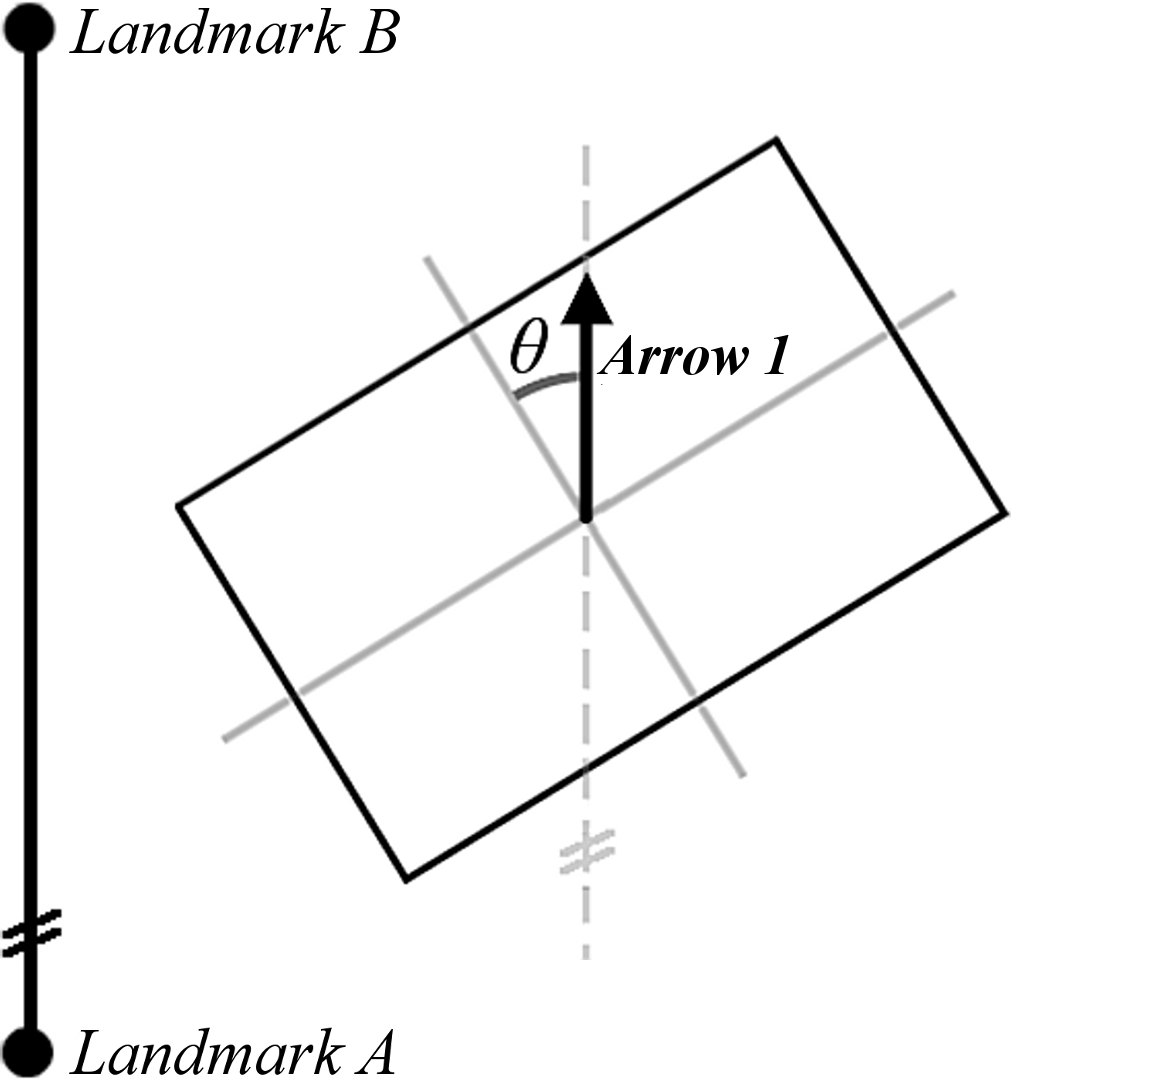
\includegraphics[width=0.4\textwidth]{figures/orientation_maths.png}
   \label{fig:orienTrig}
\end{figure}

The first of the three arrows used in the technique determines the orientation of the interface it is drawn on.
The user draws the arrow parallel to the imaginary line between the two landmarks.
The angle between this arrow and the local Y-axis of the interface, $\theta$ represents the orientation of the display as shown in Figure~\ref{fig:orienTrig}.
The user must draw this orientation arrow in the same direction on all the interfaces being located.
\textbf{$\theta$} can then be used to create a vector representing the real-world environment's Y-axis locally on the interface.
This can then be used in calculating the interface's physical position.

After drawing the orientation arrow the user is required to draw two further arrows which point directly to the landmarks (see Figure~\ref{fig:trig}).
Each of the arrows must point towards a separate landmark.
The angles of the user drawn arrows from the world's Y-axis, $\alpha$ and $\beta$, are used to determine the values used in calculating the location of the interface.
For each of these two arrow, the angle between the local y-axis of the interface and the arrow is summed with $\theta$ to derive $\alpha$ and $\beta$.

The angle between the two arrows, \textit{S}, is used in conjunction with the angle between one of the arrows and the local representation of the real world environment's Y-axis, \textit{T}, to determine the location of the interface.
Algorithm~\ref{algo:location} outlines the calculations involved in determining the \textbf{x} and \textbf{y} values of the interface's centre point in the physical environment.
The resulting values are relative to Landmark A's position shown in Figure~\ref{fig:trig}.

\begin{figure}[h]
   \centering
   \caption{Calculation of a interface's location.}
   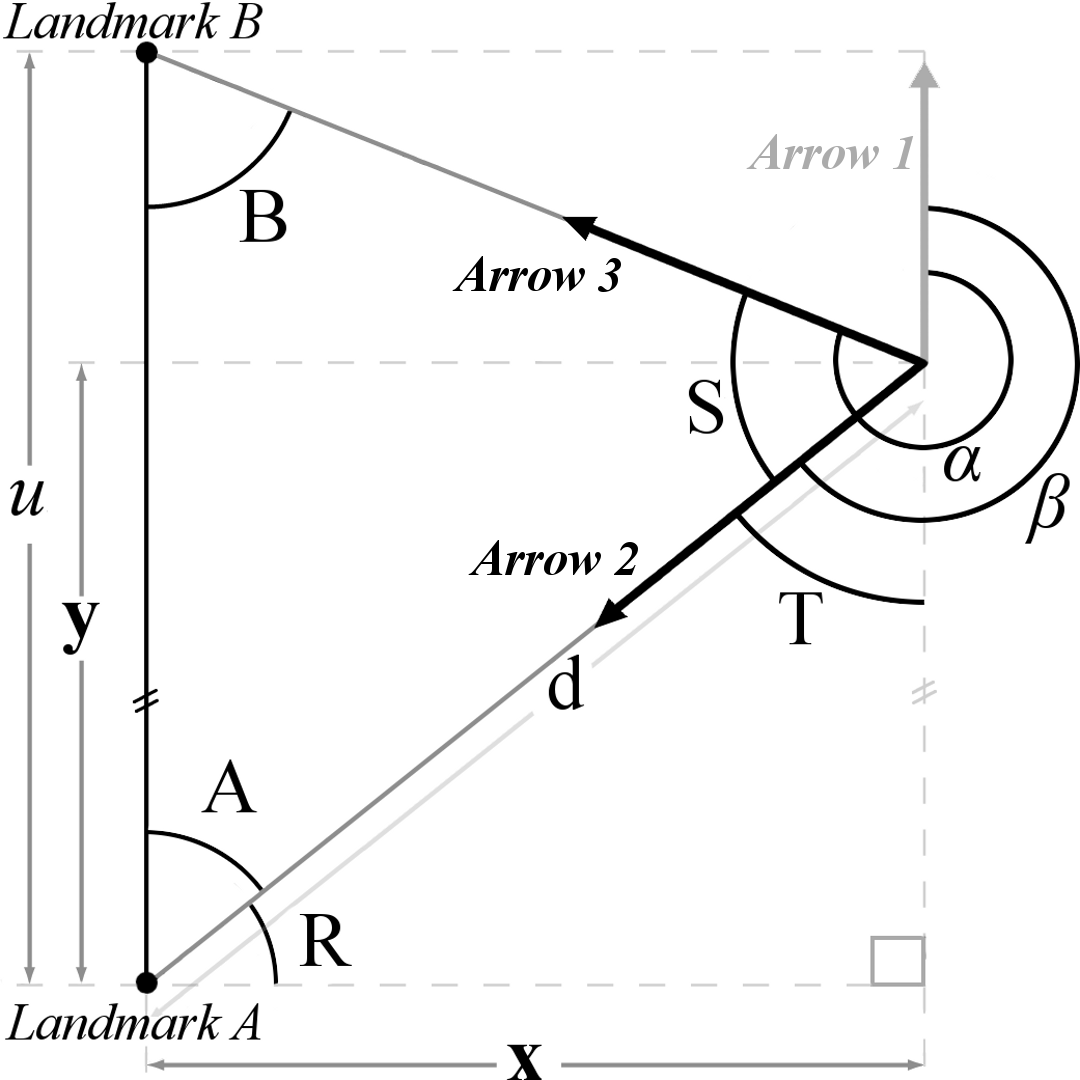
\includegraphics[width=0.475\textwidth]{figures/trig-illustration.png}
   \label{fig:trig}

\begin{Algorithm}{6cm}
\caption{Calculating the location of an interface.}
\label{algo:location}
\begin{algorithmic}
\STATE \textbf{getLocation}(${\alpha}, {\beta}$)
\INDSTATE[2] S = $\alpha - \beta$
\INDSTATE[2] T = $\beta$ - 180\degree
\INDSTATE[2] R = 90\degree - T
\INDSTATE[2] A = 90\degree - R
\INDSTATE[2] B = 180\degree - S - A
\INDSTATE[2] d = $\sin (B) * (u\ / \sin (S))$
\INDSTATE[2] x = $\sin (T) * (d\ / \sin (90\degree))$
\INDSTATE[2] y = $\sin (R) * (d\ / \sin (90\degree))$
\STATE \textit{return}\ x, y
\end{algorithmic}
\end{Algorithm}
\end{figure}

This technique has a number of benefits over the alternatives of sensing technologies and direct measurements.
The technique only needs one known value before use; this is the distance between the landmarks.
Since it is a requirement of the technique that these landmarks are not moved, this value will not need to be re-measured.
Therefore the technique can be performed relatively quickly once this measurement is obtained in comparison to measuring the locations of the interfaces directly.
This ability to be performed quickly without the need for repeated, time consuming measurements makes the technique suitable for any scenarios where the interfaces may be moved regularly.
Because of this the technique can be deemed \textit{quick}.

Because the technique does not rely on any additional technologies there is no additional cost for its implementation into a system.
This independence from additional hardware ensures that the technique is \textit{inexpensive} and \textit{not encumbering}.
Also, due to the technique's dependence on user inputs, rather than technologies, it is made suitable for use in environments where there may be many obstructions, such as the users themselves, around the interfaces.
If any immovable obstructions are present in the physical space between the interface and the reference points, a user can utilise their knowledge of the environment to make an informed placement of an arrow.
Therefore the technique can be deemed \textit{obstruction tolerant}.

The technique's design does allow for its use on interfaces which do not utilise direct-touch inputs.
However, the ability to directly manipulate the arrows may be advantageous when trying to achieve an alignment between an on-screen arrow and a physical landmark. 
The act of aiming towards reference points allows for a form of direct feedback where the user can adjust the arrow until they believe they have the correct alignment.  
An indirect input device may draw a user's attention away from the interface, interrupting their concentration when aligning the arrows with landmarks.
The technique's suitability for direct-touch interfaces is enhanced by the fact that text entry, which would be required with other user input based techniques, through touch interfaces can be inaccurate due to the lack of tactile feedback they offer~\cite{Weiss2009}.

This technique is obstruction tolerant, quick, inexpensive and not encumbering.
However, its dependence on the accuracy of a user's judgement of direction has the implication that the locational information it produces may not be \textit{accurate}.
The inaccuracies in a user's input into the technique will result in the calculated position of the interface deviating from the interface's actual location.
This deviation between the calculated and actual interfaces locations could make this technique too inaccurate for use in some scenarios.
Therefore, it is important to discover how a user's inaccuracies when performing the technique affect the resulting value.



%%%%%%%%%%%%%%%%%%%%%%%%%%%%%%%%%%%%%%%%%%%%%%
%%                                          %%
%% Backmatter begins here                   %%
%%                                          %%
%%%%%%%%%%%%%%%%%%%%%%%%%%%%%%%%%%%%%%%%%%%%%%

\begin{backmatter}

\section*{Competing interests}
  The authors declare that they have no competing interests.

\section*{Author's contributions}
    Text for this section \ldots

\section*{Acknowledgements}
  Text for this section \ldots

%%%%%%%%%%%%%%%%%%%%%%%%%%%%%%%%%%%%%%%%%%%%%%%%%%%%%%%%%%%%%
%%                  The Bibliography                       %%
%%                                                         %%
%%  Bmc_mathpys.bst  will be used to                       %%
%%  create a .BBL file for submission.                     %%
%%  After submission of the .TEX file,                     %%
%%  you will be prompted to submit your .BBL file.         %%
%%                                                         %%
%%                                                         %%
%%  Note that the displayed Bibliography will not          %%
%%  necessarily be rendered by Latex exactly as specified  %%
%%  in the online Instructions for Authors.                %%
%%                                                         %%
%%%%%%%%%%%%%%%%%%%%%%%%%%%%%%%%%%%%%%%%%%%%%%%%%%%%%%%%%%%%%

% if your bibliography is in bibtex format, use those commands:
\bibliographystyle{vancouver} % Style BST file (bmc-mathphys, vancouver, spbasic).
\bibliography{hccis2017}      % Bibliography file (usually '*.bib' )
% for author-year bibliography (bmc-mathphys or spbasic)
% a) write to bib file (bmc-mathphys only)
% @settings{label, options="nameyear"}
% b) uncomment next line
%\nocite{label}

% or include bibliography directly:
% \begin{thebibliography}
% \bibitem{b1}
% \end{thebibliography}

%%%%%%%%%%%%%%%%%%%%%%%%%%%%%%%%%%%
%%                               %%
%% Figures                       %%
%%                               %%
%% NB: this is for captions and  %%
%% Titles. All graphics must be  %%
%% submitted separately and NOT  %%
%% included in the Tex document  %%
%%                               %%
%%%%%%%%%%%%%%%%%%%%%%%%%%%%%%%%%%%

%%
%% Do not use \listoffigures as most will included as separate files

% \section*{Figures}
%   \begin{figure}[h!]
%   \caption{\csentence{Sample figure title.}
%       A short description of the figure content
%       should go here.}
%       \end{figure}

% \begin{figure}[h!]
%   \caption{\csentence{Sample figure title.}
%       Figure legend text.}
%       \end{figure}

%%%%%%%%%%%%%%%%%%%%%%%%%%%%%%%%%%%
%%                               %%
%% Tables                        %%
%%                               %%
%%%%%%%%%%%%%%%%%%%%%%%%%%%%%%%%%%%

%% Use of \listoftables is discouraged.
%%
% \section*{Tables}
% \begin{table}[h!]
% \caption{Sample table title. This is where the description of the table should go.}
%       \begin{tabular}{cccc}
%         \hline
%            & B1  &B2   & B3\\ \hline
%         A1 & 0.1 & 0.2 & 0.3\\
%         A2 & ... & ..  & .\\
%         A3 & ..  & .   & .\\ \hline
%       \end{tabular}
% \end{table}

%%%%%%%%%%%%%%%%%%%%%%%%%%%%%%%%%%%
%%                               %%
%% Additional Files              %%
%%                               %%
%%%%%%%%%%%%%%%%%%%%%%%%%%%%%%%%%%%

% \section*{Additional Files}
%   \subsection*{Additional file 1 --- Sample additional file title}
%     Additional file descriptions text (including details of how to
%     view the file, if it is in a non-standard format or the file extension).  This might
%     refer to a multi-page table or a figure.

%   \subsection*{Additional file 2 --- Sample additional file title}
%     Additional file descriptions text.


\end{backmatter}
\end{document}
